\documentclass[a4paper,smallheadings,11pt,oneside,bibliography=totoc]{scrreprt}
\addtokomafont{disposition}{\rmfamily}
\usepackage[utf8x]{inputenc}
\usepackage[english]{babel}
\usepackage{amssymb}
\usepackage{amsthm}
\usepackage{amsmath}
\usepackage[dvipsnames]{xcolor}
\usepackage{graphicx}
\usepackage{microtype}
\usepackage{palatino}
\usepackage[round,colon]{natbib}
\usepackage[hidelinks]{hyperref}
\usepackage[titletoc]{appendix}
\usepackage{pgfplots}
\pagestyle{headings}
\usepackage{parskip}
\usepackage{tikz-uml}
\usepackage{tikz}
\usepackage{tcolorbox}
\usepackage{longtable}
\tcbuselibrary{listings,skins}
\usetikzlibrary{calc}

\usetikzlibrary{arrows.meta}
\usetikzlibrary{chains}
\usepackage{epstopdf}
\newcommand{\comments}[1]{\textcolor{OliveGreen}{[\emph{#1}]}}

\graphicspath{{images/}}
\newcommand{\cisco}{cisco_images}
\newcommand{\ciscoImageScale}{0.7}

\setcounter{secnumdepth}{3} 
\setcounter{tocdepth}{3}

% Custom fonts
\newenvironment{console_font}{\fontfamily{pcr}\selectfont}{\par}
\newcommand*{\code}{\ttfamily\selectfont}

\definecolor{codegreen}{rgb}{0,0.6,0}
\definecolor{codegray}{rgb}{0.5,0.5,0.5}
\definecolor{codepurple}{rgb}{0.58,0,0.82}
\definecolor{backcolour}{rgb}{0.95,0.95,0.92}
 
\lstdefinestyle{mystyle}{
    commentstyle=\color{codegreen},
    keywordstyle={\bf \color{blue}},
    numberstyle=\tiny\color{codegray},
    stringstyle=\color{codepurple},
    basicstyle=\footnotesize\ttfamily,
    breakatwhitespace=false,         
    breaklines=true,                 
    captionpos=b,                    
    keepspaces=true,                 
    numbers=left, 
    columns=fixed,                                   
    showspaces=false,                
    showstringspaces=false,
    showtabs=false,                  
    tabsize=7,
    language=Python,
    numberstyle=\tiny, 
	numbersep=8pt
}

%Used to format code listings
\newtcblisting{Code}[2][]{
	top=0cm,
	bottom=0cm,
	left=0.5cm,
	right=0cm,
	colback=white,
	colframe=black,
    arc=1pt, outer arc=1pt,
    listing only, 
    listing style=mystyle,
    title=#2,
    #1
}


\begin{document}

	%Title Page
	\title{Compromised and Degraded Network Simulation}
	\newcommand{\reporttype}{Final Report}
	\newcommand{\degreetitle}{BSc}
	\newcommand{\progname}{Computer Science}
	\author{Aidan Fray}
	\newcommand{\wordcount}{X}

	% Document format
	%\makeatletter
\begin{titlepage}

\vspace*{-5em}
~~

\vfill

\begin{center}
{\huge \textbf{\@title}}\\
\vspace*{1em}
{\LARGE \textbf{\reporttype{}}}\\
\vspace*{2em}
{\Large Submitted for the \degreetitle{} in}\\
\vspace*{0.5em}
{\Large \progname{}}\\
\vspace*{2em}
{\Large \today}\\
\vspace*{2em}
{\Large by}\\
\vspace*{2em}
{\Large \textbf{\@author}}\\
\vspace*{3em}
{\large Word Count: \wordcount{}}
\end{center}

\vfill
\begin{center}
	
\includegraphics[height=0.075\textheight]{title_page/UoH_Logo.pdf}
\end{center}

\end{titlepage}
\makeatother		
	\newpage
	%\tableofcontents
	\chapter{Introduction}
Networks and their functionality play a crucial role in today's internet infrastructure. Networks relay packets and allow communication between computers from opposite sides of the globe. This paper will discuss and explore the effects of degradation on a live network, and how these effects can be reduced or negated. 

The live network will be a simulation of network traffic, which will be routed through a custom router running on a small Raspberry Pi. This Raspberry Pi will run the degradation tool that will allow the control of network conditions. 

Issues may arise from various aspects of the project. Firstly the accuracy in simulation of network traffic may cause inaccuracies in the tool's validity. More problems may occur regarding the discovery of effective practises to negate hostile network conditions, and other issues involve the stability and scalability of the tool meaning that its maximum capacity needs defining. These issues will be discussed later.

	%This section should define the overall aim of the project and clearly state the individual, measurable objectives that you have set for the project (objectives should have a deliverable outcome associated with them). In short, this section should clearly identify exactly what it is that you are intending to achieve in the project.
\chapter{Aims and Objectives}
\begin{center}
"Create a custom simulated network that can demonstrate and visualise network degradation and common DoS attacks, this is so network engineers can identify weak spots and points of strain"
\end{center}


The above aim will be achieved by reaching these targets:

%---------------------- OBJECTTIVE 1 ----------------------- %
\paragraph{Objective One}
Develop a fully working clients and servers that communicate using HTTP/1.1 \citep{HTTP} and FTP over the TCP protocol alongside a client and server that use the UDP protocol

\begin{itemize}
\item The client will use HTTP/1.1  over TCP and will need to be able to send PUT and GET requests to the server.
\item The server will need to be able to deal with HTTP/1.1 requests and act accordingly. This means when the server receives a PUT request it will alter data. A GET request will therefore mean a retrieval of data. 
\item The client will need to be able to upload and download files using FTP.
\item The server should be able to have files uploaded to it and send data when a download is requested.
\item The UDP client will need to send a set number of packets each containing a single value that increments with each packet sent.
\item The UDP server will display a grid of received and missing packets where the positions are denoted by the packets value, this will give a visual representation of missing packets.
\end{itemize}  

The functionality above with be contained in one executable that will take parameters to define which client or server will be loaded. For example the parameters '-f c' will load the FTP client.

Note: Authentication for any of these channels is outside the scope of this project

\label{sec:obj2}
%---------------------- OBJECTTIVE 2 ----------------------- %
\paragraph{Objective 2}
Create a program that runs on a Linux based OS that can be used to simulate degradation and attacks. This program will then be run on the router.

\begin{itemize}
\item Degradation factors will be:
	\begin{itemize}
	\item Packet loss
	\item Latency
	\item Rate of transfer (Bandwidth)
	\end{itemize}
\item Attacks will compose of some small and simple attacks; Possible attacks could be:
	\begin{itemize}
	\item UDP Flooding \citep{xiaoming2010denial}, where the network is filled with erroneous packets that will attempt to clog up the network.
	\item ARP (Address Resolution Protocol) spamming and poison, the network is filled with ever changing ARP requests that cause computers to not be able to correctly resolve the 	valid locations of each other (Whalen, S., 2001).
	\item TTL (Time to Live) incrementing where packets will eventually end up in loops and cannot die, causing a “packet storm”.
	\item There may also be space for other attacks if time allows.
	\end{itemize}
\end{itemize}

%---------------------- OBJECTTIVE 3 ----------------------- %
\paragraph{Objective 3}
Create a working custom router that can be used to simulate degradation in conjunction with the program outlined in Objective 2

\begin{itemize}
\item This router should be able to act in place of a real commercial router. 
\end{itemize}
Note: The speed that the router can handle is not a concern.
\begin{itemize}
\item This router will have to be able to deal with internet connections over Ethernet and a wireless connection, with multiple devices connected at the same time.
\end{itemize}
Note: The security of the router is also outside of the scope of this project


	%This is a narrative description of the general context within which your project fits. Depending on your particular project characteristics, you are required to include discussion of any or all of the following – previous related work; the work or objectives of a client; the essential principles of systems or techniques you are using.%

%All this narrative should be properly referenced to source material citations. Remember that a high class project will refer to background sources beyond just those on the Web. %

%In writing this section you should pay close attention to your audience and their prior knowledge of the subject(s) that you are discussing. You should assume that your reader is a student who has just completed the second year of your degree programme and can therefore assume that the reader is familiar with all topics taught up to the end of the second year. Anything that is needed to understand your project and its context but which has not been taught by the end of the second year of your degree should be discussed in this background section. %

%This section may include one or more of the following subsections. It is difficult to give prescriptive guidance on which subsections you should include as this depends on the nature of the project you are undertaking – you should discuss this with your supervisor.%
\chapter{Background}

%Problem Context:
%If your project involves significant work on a non-computing topic that is likely to be unfamiliar to most readers (e.g. linguistics, fluid dynamics) you should describe the important principles, concepts and terminology of that subject area in some detail. You will have had to learn these yourself in getting to grips with this unfamiliar topic and you should summarize what you learnt to enable the reader to understand your subsequent discussion on your project work and how this relates to the wider topic area.
\section{Problem Context}

The main focus of this project is to create a network degradation tool that can be used to simulate imperfect network conditions. To understand the goal better it is important to know what criteria reduce network quality.

Latency, packet loss and bandwidth are the main factors that distinguish between good and bad internet connections. Latency is the delay between sending a message and seeing its result. Packet loss is the percentage of packets that are lost in a transmission, the higher the percentage, the more effect it has on the speed and stability of the network. Bandwidth, is the measure of how many bits/bytes are being transferred per second, the larger the bandwidth the more data can be transferred in less time, thus making the overall connection faster. A combination of favourable values from these criteria defines a good network connection. One way to visualise the throughput of a network connection is a download and upload and speed test, the result of these is measured in Mbps and can be used to quickly compare the speed of two connections, this will be used later to briefly show the degradation.

Other small signs of poor network conditions is Jitter and Error rate. Jitter is simply the variance in packet delays, this is normally a issue that exists in large packet switched networks, this is however not an issue in TCP/IP based communications because TCP protocol deals with these issues. However, VoIP (Voice over IP) that uses UDP as its transport level protocol is visibly degraded by heavy jitter. Error rate is the number of bit errors that have occurred in a data stream over a period of time. This can again effect UDP based communications heavily but the TCP protocol deals with these issues so remains relatively unaffected.

It is also necessary to mention the protocols that are to be used in the network simulation section. TCP \citep{TCP} and UDP \citep{UDP} are the transport layer protocols up for discussion. 

\comments{Talk about how TCP deals with jitter?}
\comments{Talk more about Packet Loss/Latency/Packet Loss maybe even about smaller signs of bad connection quality?}

\subsection{Protocols}
\subsubsection{Transport Control Protocol (TCP)}
TCP's main design choices are centred around reliability, where it has a few techniques designed to make sure packets arrive correctly. 

\begin{center}
	\includegraphics[scale=0.7]{TCP_header}
	\begin{figure}[h]
		\caption{TCP Header (RFC 793)}
	\end{figure}	
	
\end{center}

\subsubsection*{Initiating a connection}
The connection begins by being initiated with a series of signals where they are abbreviated as ACK (Acknowledgement) and SYN (Synchronise). The initiating party begins by sending an empty packet with the SYN flag set, this starts the synchronization process. Then once the target computer receives this SYN packet it sends back and ACK and its own SYN to the initiating computer (This is normally send a single ACK + SYN packet). Where finally the initial computer sends back an ACK packet for the previous SYN packet, this connection has now been initiated and the communication channel has been set up. This process is known as a `3-way handshake'.

For TCP to remain reliable it needs to maintain data on the status of a connection. A connection is uniquely identified by the pair of sockets that define the two end points of the connection. The information retained for each connection is: sequence number, acknowledgement numbers and window sizes. These values are used to calculate the expected next packet to therefore detect if errors have occurred in transmission.

\begin{center}
	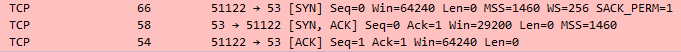
\includegraphics[scale=0.8]{SYN-ACK}
	\begin{figure}[h]
		\caption{The output from Wireshark showing the handshake}
	\end{figure}
\end{center}


\subsubsection*{Sequence Numbers and Acknowledgement Numbers}
One of the main mechanisms for detecting missing and incorrect packets is the sequence and acknowledgement numbers. The TCP design states that every octet (byte) will have a corresponding sequence number, this sequence number is then increased by the size of every transmitted packet, the length of a packet can be calculated by taking the total size of the packet and taking away the size of the header. For example, if a packet with a length of 100 was sent it would move the sequence value up by 100, this gives the protocol the information to judge what it should be expecting and what it has received, and if those two values don't add up an error has occurred. 

The guarantee arrival the sender needs to know its packets have been received, this is where the acknowledgement number comes in, packets carrying acknowledgements are known as ``ACKs". For a packet with a sequence number of 100 being sent will require a packet to be send back containing the ACK number of 100 to verify that is has been transferred correctly, an ACK packet is signified by the `ACK' flag in the packets header. If the ACK packet isn't received before the the time-out value has been reached the packet is resent, this is how TCP guarantees retransmission of packets and it's also one of the reasons why packet loss doesn't have the same effect it does on UDP with TCP.

In situations where connections are created and recreated quickly in succession or are being quickly re-established after errors there cannot be sequence numbers that clash with previous segment that may still exist on a network connection, therefore TCP solves this issue by generating new initial sequence numbers using a Initial Sequence Number (ISN) generator that uses a 32 bit clock, this clock has a life cycle of 4.55 hours where this time period is commonly known as the Maximum Segment Lifetime (MSL) and if a ISN is generated within this time is can be guaranteed to be unique.

\subsubsection*{Receiving Window}
In the TCP header there is a two byte value that represents the receiving window size, this value defines the maximum size of unacknowledged packets the receiving end has space for. So if a client sends a packet with a 65535 window size value it tells the receiving computer not to send more than 65535 bytes before receiving corresponding acknowledgements. This value can also be extended using a value in the area allocated in the `TCP Options' called `windows scaling', this allows the value in the window size to be multiplied by this scale value. So, for example a window size of 65535 with a window scale of 5 would have a total window size of 327675 Bytes. This means that the larger the window the more data can be send before the protocol needs to wait and can normally mean faster transfer speeds. Please note, this exchange of window scaling values is only performed in the handshake and can only be present in the initial exchange of packets.

\subsubsection*{Flow Control}
Flow controls is a mechanism used by the protocol to ensure that the receiving party does not become overwhelmed by the incoming transmission of packets. TCP has two types of buffers the `send' and `receive', where the send buffer collects what data is going out and the receive buffer collects what is coming in. This goal of the flow control is to prevent the sending of packets that will not fit in the destination receive buffer and therefore will prevent these packets from being dropped. The protocol achieves this by allowing each party to advertise its available receive buffer space through a this window size section in the header that was discussed previously. (This is included in each ACK packet). Once the receive buffer is full the receiving party will advertise what is known as a 'zero window' where it sets the window size to `0' and transfer will stop until there is free space in the receive buffer.

\subsubsection*{Sliding Window}
To control the number of packets the protocol has in flight at any one time the protocol utilises the `sliding window. The size of the sliding window is altered by two factors: The size of the send buffer and the size of the destinations receive buffer, therefore the maximum amount of data the protocol can send is the smallest of the two previous values. The sliding window then dynamically works out how many packets it can send by working out the maximum data it can send while keeping track of the number of packets in flight (unacknowledged) and the current window size. This whole process gives the protocol the ability to dynamically adapt to changing conditions and prevent buffers from being overfilled the receiving end.


\subsubsection*{Congestion control}
When there are situations where multiple clients are connected to one receiver lets say a router for this example, the bandwidth needs to be split between the number of clients and this is performed by congestion controls. The clients send data and keep increasing their transfer rate until they discover packet loss, packet loss in this case is assumed to be a sign of congestion - this is because it thinks the packets are being lost because the router is dropping them due to insufficient packet buffering space. So as the number of clients requesting data from the router is reduced more bandwidth is freed up and available, the congestion algorithm is periodically probing the network to check for available bandwidth by increasing it transfer rate until packet loss is encountered where it then slows down and repeats the process. This results in TCP auto balancing when new clients are introduced and utilizing as much bandwidth as is available. Later this report will discuss the effects of packet loss, latency and other degradation signs on this congestion control.

\subsubsection*{Congestion Algorithms}
%TODO Talk here about common congesting algorithms and how they work - This will be great to talk later in the experiementation section


\subsubsection*{Closing a connection}
The closing of a TCP connection is very similar to the initial construction of a TCP connection, but in this case the protocol utilises the `FIN' flag defined in the TCP header. In this example it will be a client disconnection from a server. After all the data is transferred the client no longer requires a connection to the server and sends an empty packet with the FIN bit send, the server receives the packet and returns an ACK. The server now sends its own FIN and this is then acknowledged by the client. This middle step with the server sending an ACK and FIN separately is performed in a single packet in live networks. The client and server not know the connection is closed and will free up any resources allocated to that connection.

\clearpage
\subsubsection{User Data Protocol (UDP)}
\begin{center}
	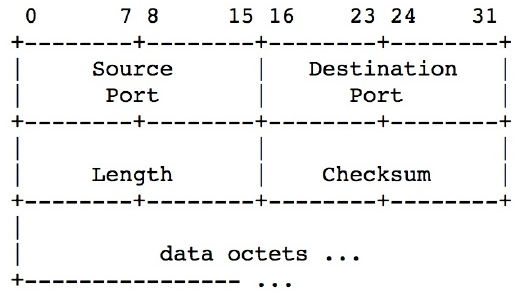
\includegraphics[scale=0.7]{udp_header}
	\begin{figure}[h]
		\caption{UDP Header (RFC 768)}
	\end{figure}		
\end{center}

UDP is by design the opposite of TCP and often you'll find the two protocols compared. UDP is often referred to as ``fire and forget" \citep{kempf2011thoughts} this is a short way of describing how UDP deals with packets. When a packet is to be sent UDP sends the packet and moves onto the next. However, this means aside from the checksum in the UDP header (A checksum can be used to check that the UDP data has been transferred correctly) there is zero error checking for the UDP protocol and results in UDP being considered unreliable in comparison to TCP. 

This lack of error-checking overhead however, greatly improves the speed of UDP protocols. UDP is not used in situations where communication is vital, but does find itself implemented in examples like voice or video chat because errors in these services are not catastrophic to operation and these imperfections can even go unnoticed.

\comments{Speed comparison between UDP and TCP}

As the very small UDP header shows, it is a very simple protocol and is effectively a thin wrapper on top of the IP layer that allows for very quick transfers but with the cost of un-guaranteed reliability, this is why packet loss effects UDP massively and this overall effect will be fully disused later.

\clearpage
\subsubsection{Address Resolution Protocol (ARP)}
The tool will be deployed either by having it run on a small custom computer set up to act as a router for the synthetic test network or by jumping between a user and an actual router on a live network. The program will achieve this jumping between a user and the router by utilising a long term vulnerability in the Address Resolution Protocol (ARP) \citep{arp2001}, before this is explained further it is first important to understand the relevant parts of a local network.

Each computer on a Local Area Network (LAN) has an IP assigned to it, this is the identifier on the local network, with this each computers wireless card has a MAC address, a MAC address is a unique identifier for a computer and is used to link up this non-unique local address (IP) to a real computer on a network, this combination of IP address and MAC address allow for the reuse of local IP numbers. The ARP protocol is therefore used to find out what MAC address is associated with a local IP address and visa versa. This is achieved via an entire network broadcast where computers that don't match ignore the ARP request, and the one being requested sends back a reply containing it's MAC address. Each computer maintains its own version of the arp data known as its 'ARP cache'.

An ARP packet is a very simple message format that contains an operation code that can either can be a request (1) or a response (2) where the packet also contains 4 addresses - 2 pairs of hardware and protocol addresses for the sender and target.

The ARP protocol contains no form of authentication verification meaning a malicious computer can send out faked custom ARP requests to change specific values in the routers ARP table, meaning a computer running this software can appear as the router to the victim, while also appearing as the victim to the router, thus having all the traffic between the two routed through the attacking computer. 

\begin{center}
\newcommand{\tgap}{0.1cm}

\begin{center}
\begin{tikzpicture}[
	every node/.style={fill=white},
    diagram item/.style={},
    align=left
]         

\node (Router)[
    diagram item,
    label=above:Alice,
    yshift=-2cm
] {
\includegraphics[scale=\ciscoImageScale]{\cisco/workstation}};

\node (Victim)[
	diagram item,
	label=above:Bob,
	right of=Router,
	xshift=7cm
] {
\includegraphics[scale=\ciscoImageScale]{\cisco/workstation}};

\node (Attacker)[
	label=below:Eve,
	below of=Victim,
	xshift=-3.5cm,
	yshift=-3.5cm
] {
\includegraphics[scale=\ciscoImageScale]{\cisco/laptop}};

\draw[-] (Router)--node[yshift=0.5cm]{Old Connection}(Victim);
\draw[red, very thick] (Router)--node{New Connection}(Attacker);
\draw[red, very thick] (Attacker)--node{New Connection}(Victim);


\end{tikzpicture} 
\end{center}


	\begin{figure}[h]
		\caption{Photo depicting a MITM attack}
	\end{figure}
\end{center}

\subsubsection{Custom Router - Raspberry Pi}
As mentioned previously the effects will be performed on a custom computer acting as the router, because the network will be set-up to pass all traffic through this router, it will be able to simulate degradation on the entire networks traffic.
The Raspberry Pi \citep{upton2014raspberry} has been decided as the choice for the small custom computer. Originally designed to teach children to code on an inexpensive (less than £30) computer, the Pi has found itself involved in a multitude of uses ranging from NAS (Network Attached Server) to robot controllers. This is useful in this project due to its ease to set-up as a router, this is because of the easy access of low level aspects of the operating system due to it running a based OS. The Raspberry Pi will be run with its default Raspbian OS \citep{pi2014raspbian} that is built upon Debian \citep{murdock1994overview}. This is a optimised OS for the internal ARM CPU that allows the Raspberry Pi to run modern stripped down programs on its very limited hardware, where it will have plenty of power to easily handle traffic as a router.

\subsubsection{Router alternatives}

\subsubsection*{MinnowBoard}
MinnowBoard \footnote{\url{https://minnowboard.org/}} is a company specialising in open source custom made processing units designed to remain compact while still being able to perform relatively heavy computation. Even their basic options have more RAM and processing speeds compared to that of the Raspberry Pi, but this comes at a higher cost the basic model retails in at £110 more than 3 times to price of the Raspberry Pi. The increased processing speed would be the total bandwidth the router could handle would be increased and could even allow the GUI as an alternative to the command line, but this extra cost and increased processing speed don't add any extra value to the goal of the project and therefore the option was discarded.

\subsubsection*{Commercial router}
A commercial out-of-the-box router could be used with a custom version of OpenWrt \footnote{\url{https://openwrt.org/}}. OpenWrt is a custom version of Linux that is designed for embedded devices. To install this version of Linux on a router would require `flashing' the software, flashing is the process of overwriting the embedded EEPROM or other type of embedded memory with the firmware of your choice, this process is lengthy and has no guarantee of working. This process however would provided me with a device that could run the degradation script that is fully designed to function within a network, this could possibly mean faster processing speeds and a smoother experience. However due to the uncertain set-up time compared to that of the Raspberry Pi this option was decided against, this however could be an aspect to implement in the long term improvements, this will be further discussed later in the report.

\comments{Talk here about alternatives to the raspberry pi}

%Comparison of Technologies:
%If there are several possible technologies that could be used in your project work you should present a comparative analysis and critical appraisal of each of these technologies. You should create a subsection for each of the technologies you discuss and title each subsection with the name of the technology it describes (e.g. object-oriented databases, XML ). Within each subsection you should provide an overview of the technology, its key features and its strengths and weaknesses in relation to your project.
\section{Comparison of Technologies}

\subsection{Protocol Comparison}
\subsubsection{TCP Based Protocols}

\subsubsection*{HTTP}
TCP has various protocols built on top of it. One of the most widely used protocols is HTTP/1.1 \citep{HTTP}. HTTP is a structured language used to transfer data worldwide. Its main use is the movement of web based data, this has been chosen as one of the protocols to be used in the test network to simulate live real-world traffic, this is due to the protocols heavy use in the real world. The protocol will be utilised by a web browser that attempts to access a web page, the degradation will therefore be visible through how quickly the web page loads and how responsive the connection seems.


\subsubsection*{FTP}
Another protocol based on top of TCP is FTP (File Transfer Protocol) \citep{FTP}, and as the broken down acronym suggests is the protocol used to transfer files across a network. This protocol has been selected also due to its integral use in a live network. It also has a quite intuitive way of representing the speed of a network through a download speed that is easy to understand for most users. The protocol will be tested with dummy files ranging from 1MB to 5GB. This size range was chosen to fully cover the normal spectrum of file size where it roughly ranges from a Word document to high quality video.

\subsubsection{Other TCP Considerations}

\subsubsection*{SFTP}
SFTP (SSH File Transfer Protocol) \citep{SFTP} was a consideration as a protocol to be used for the demonstration purposes. SFTP effectively is a secure version of FTP (but not to be mixed up with the Simple File Transfer Protocol). This was decided not to be used because of its added features such as authentication security does not fit within the scope of the project, and does not relate to network degradation. 

\subsubsection*{Mail based protocols}
Another widely used set of protocols are the email based family of protocols. SMTP (Simple Mail Transfer Protocol) is involved in the sending of mail, while examples like IMAP/POP are used for receiving mail. These protocols use TCP as their transport layer protocols. These protocols are fundamental to email functioning on the internet but visualisation into their degradation would be not different to that of bare TCP, the implementation of an email client would add unnecessary complexity while offering almost zero added value to the demonstrative purposes of this project.



\subsubsection{UDP Based Protocols}
UDP due to its speed but inherent unreliability, UDP is hugely affected by packet loss. Therefore, the effects on UDP has decided to be visualised by a program that simulates image transfer by assigning an individual UDP packet a number that corresponds to a single pixel, this packet is then sent. Once the server receives the packet, it reads the pixel number stored in the packet and changes that specific pixel to green. This creates a matrix of red (lost) and green(received) pixels. This therefore, gives a simple but effective visualisation of packet loss. 

\begin{center}
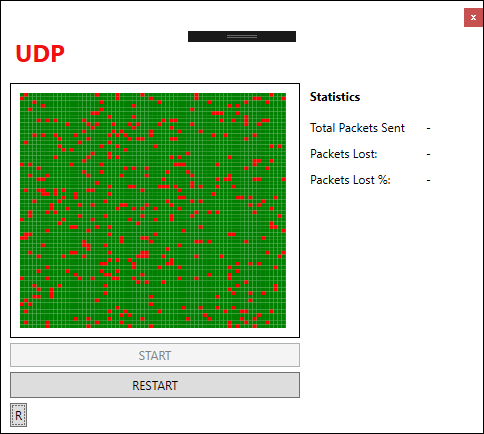
\includegraphics[scale=0.7]{UDP-Demo}
	\begin{figure}[h]
		\caption{Initial draft of the UDP user interface}
	\end{figure}
\end{center}

Other effects can also be performed on UDP to measure the degradation, latency and the arrival order of the packets are big signs of hostile transfer conditions. The monitoring of the latency and order can be performed by the UDP interface and could provide a much more detailed overview of the current health of the connection.

\subsection*{Other UDP based protocols}
UDP is used for situations where speed is required but reliability is not. Media streaming is a common example, lots of data need to arrive to the client quickly where missed frames when not too large can go unnoticed. This kind of implementation would be a huge overhead and even if a 3rd party application was used set-up and debugging would utilise time while providing not much more insight into what is happening to the protocol when degradation is high. This is why UDP had been left as bare boned as possible and the protocol has been left relatively exposed to allow an effective way to visualise the effects.

\subsection{Operating Systems}

\subsubsection{Linux}
Linux is the broad definition of a family of computer operating systems. The defining characteristics of a ``Linux" OS is the free and open source approach and the use of the Linux Kernel. Android for example has the largest market share in the mobile OS market \citep{share2015desktop}, Android utilises the Linux kernel as the centre for its operating system.

Linux was chosen for this project for its open source element that allows easy access to low-level features in the kernel. The section of the kernel that deals with the filtration of packets for uses like firewalls and packet sniffers is referred to as the ``NetFilter". This acts as an API of sorts where packets can be routed to the net-filter queue to await a verdict (accept or drop) before being moved on. This is the basis for the functionality of the program, it will run on the Raspberry Pi and route all packets that enter the box to the queue where the program will perform its effects on the packets. Latency for example is one of the simplest effect to simulate, the packet will be routed into the queue, taken out and stored and the delay between storing and accepting will be the set latency value and therefore simulating the effect of latency on that packet.

\subsubsection{Windows}
Linux was chosen over the other possible alternative; Windows. The Windows OS is distributed as closed source software under proprietary licences meaning to understand what is happening under the hood is far more difficult. The operating system is documented well and there is support for this form of functionality. Windows does provide a solution to the packet filtering in the same way that NetFilter does, it's called Windows Filtering Platform (WFP) and it is a an API that allows access to the systems services in order to provide to create packet filtering application. Its functionality is very similar to that of NetFilter.

Windows however was not used because of the size of the Windows OS. Below is the minimum system requirements for Windows 10 \footnote{\url{https://www.microsoft.com/en-US/windows/windows-10-specifications}}

%Windows Min System Requirements Table

\vspace{5mm} 
\begin{center}
\begin{tabular}{| l | l |}
	\hline
	Processor & 1 gigahertz (GHz) or faster processor or SoC \\
	RAM & 1 gigabyte (GB) for 32-bit or 2 GB for 64-bit \\
	Hard Disk Space & 16 GB for 32-bit OS 20 GB for 64-bit OS \\
	\hline
\end{tabular}
\vspace{5mm} 
\end{center}

This compared with the full Debian \footnote{\url{https://www.debian.org/releases/stable/i386/ch03s04.html.en}} OS that the striped down version of the Raspberry Pi's OS is based off:

\begin{center}
No Desktop\\
\vspace{1mm} 
\begin{tabular}{| l | l |}
	\hline
	Processor & 1GHZ Pentium 4 \\
	RAM & 128 MB \\
	Hard Disk Space & 2 GB \\
	\hline
\end{tabular}

\vspace{2.5mm}
With Desktop\\
\vspace{1mm}
\begin{tabular}{| l | l |}
	\hline
	Processor & 1GHZ Pentium 4 \\
	RAM & 512 MB \\
	Hard Disk Space & 10 GB \\
	\hline
\end{tabular}
\vspace{5mm}
\end{center}

The Raspberry Pi in this instance will be run with no desktop.

As you can see from the comparison above the Linux based OS has a much smaller set of requirements where RAM usage for example is 8 times smaller and therefore due to Linux's transparency and overall efficiency the OS is far more suited for us in conjunction with the Raspberry Pi.

%Alternative Solutions:
%If others have produced solutions or addressed similar problems to those addressed by your project you should describe those alternative solutions here. Similarly, if several possible approaches suggest themselves as ways of solving the problems inherent in your project you should discuss those here. You should provide a comparative analysis and critical appraisal of each alternative solution approach or existing solution, identifying their key features and their strengths and weaknesses in relation to your project.
\section{Alternative Solutions}

\comments{For all the solutions I need to be much more critical of the positives and negatives}

\subsection{clumsy}
A more modern application of network degradation is clumsy 0.2 \footnote{\url{http://jagt.github.io/clumsy/index.html}}. It provides various options (that can run in parallel) that effect network conditions. 

\begin{center}
	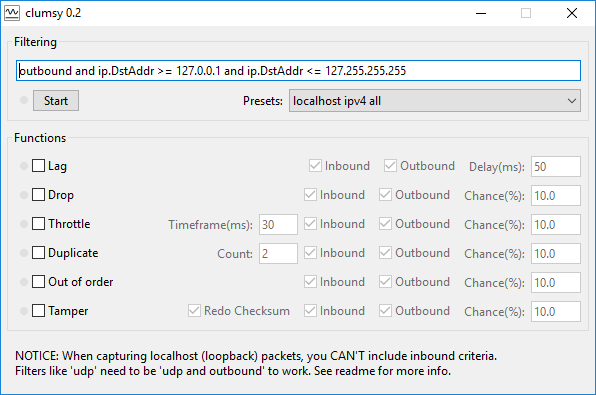
\includegraphics[scale=0.5]{clumsy}
	\begin{figure}[h]
		\caption{Main UI of clumsy}
	\end{figure}
\end{center}

The tool provides a way to affect network conditions. It solves issues involved with simulating harsh network conditions on a network. It does allow for filtering and has a couple of filter pre-sets, it however doesn't provide options to simulate live traffic and options to capture or visualise traffic is not part of the main package.

This tool provides and easy to use and simple tool that requires no extra download and can be run straight from the .exe, however this is only works on Windows machine and it uses the WFP API that was mentioned in the Windows OS section. It also only affects the traffic on the local machine, this is good for testing tools in the development stage of an application but cannot easily be used to simulate degradation across a simulated network.

\subsection{TMNetSim}
TMNetSim \footnote{\url{http://www.tmurgent.com/appv/en/87-tools/performance-tools/177-tmnetsim-quick-and-easy-network-simulation-tool}} is another tool that covers aspects of this project. Unlike clumsy TMNetSim is designed to provide degradation that expands over the network. However, to achieve this it has to be set-up on every machine, this is clunky and time consuming. The degradation script can negate this lengthy set-up with the intended inclusion of the ARP Spoofing that will allow rapid deployment of the script between target and router. Further criticism relating to the ease of use of this application, it has a large number of controls on it's interface and will involve a larger learning curve to master compared to other simpler tools, this however might be the bi-product of more functionality; increased complexity.

This tool includes very complex ways of simulating realistic degradation with ``Gausian" and ``Normal" delay modes, that attempt to provide more accurate representations of real-world delays. This is a great feature that could drastically improve the accuracy in simulating degradation and will need to be considered as an extra inclusion into this project.

%TODO - Added some more alternative solutions there should be at least two more

%Comparison of Algotithms%
%There may be a number of different algorithms which could be applied to the central problems in your project and you have had to choose which of these algorithms are the most appropriate for your implementation. If this is the case then you should provide a comparative analysis and critical appraisal of each of the potentially applicable algorithms, highlighting their key features and their strengths and weaknesses in relation to your project.%
\section{Comparison of Algorithms}



%Process and Methodology%
%If your project is concerned with improving, implementing or evaluating a particular technical process or method of working you should discuss these in detail. We are not expecting you to describe what software development methodology you are following in implementing your project and you certainly do not need to regurgitate textbook descriptions of the Waterfall method here as everyone already knows that model well.%
\section{Process and Methodology}

	%In this section you will discuss the Technical Development related to your project.
%In one or more chapters you must describe fully the design and development strategies you have adopted and the results achieved.  You may refer to appropriate User and System documentation presented as appendices to avoid repeating extensive detail, so you can focus here instead on a discussion of your reasons for adopting the techniques and strategies you have followed.

%Again, it is difficult to give prescriptive guidance on the subsection structure you might adopt, as this will depend on the nature and content of your project.  However, you will probably want at least to consider sections addressing issues of System Design; Implementation; Testing.  If there is a lot to cover in any of these areas, it may warrant presentation as a full chapter rather than a section.

\chapter{Technical Development}

% Section Description:
%
\section{Tool Architecture}
Below is the system architecture for the degradation tool:

\begin{center}
	\newcommand{\width}{3cm}
\newcommand{\imageScale}{0.2}

\tikzset{%
  >={Latex[width=2mm,length=2mm]},
  % Specifications for style of nodes:
            base/.style = {rectangle, rounded corners, draw=black,
                           minimum width=\width, minimum height=1cm,
                           text centered, font=\sffamily},
            red/.style = {base, fill=red!15},
            blue/.style = {base, fill=blue!15}}
          

\begin{center}
\begin{tikzpicture}[node distance=1.5cm, every node/.style={fill=white, font=\sffamily}, align=center]

	\node(User)[xshift=-10cm]{\includegraphics[scale=\imageScale]{User}};		
	\node(UserText)[below of=User]{User};		
	
	\node(GUI)[base, right of=User, xshift=(\width), yshift=2cm]{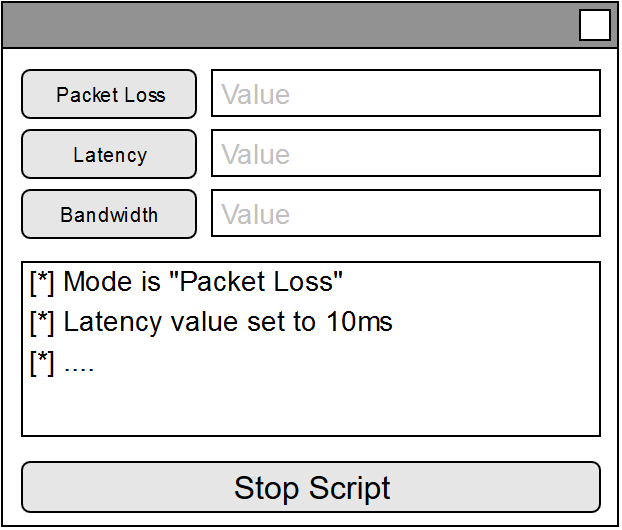
\includegraphics[scale=\imageScale]{Packet_UI_Design}};
	\node(GUIText)[below of=GUI, yshift=-0.5cm]{GUI};	
	
	\node(CLI)[base, below of=GUI, yshift=-2.25cm]{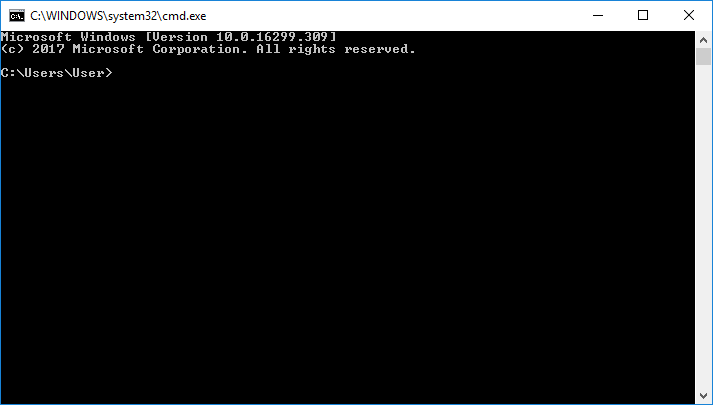
\includegraphics[scale=\imageScale]{CLI}};
	\node(CLIText)[below of=CLI]{CLI};
	
	\node(Effect)[blue, right of=User, xshift=(\width * 2) + 2cm]{Effect Choice};	
	\node(Nfqueue)[base, right of=Effect, xshift=(\width)]{NFQUEUE Creation};	
	
	\node(Parameters)[base, below of=Effect]{Parameter Handling};	
		
	
	\node(Packet)[red, below of=User, xshift=2cm, yshift=-4cm, text width=6cm]{Incomming Packets pushed into the NFQUEUE};
	\node(ChosenEffect)[blue, right of=Packet, xshift=\width + 2cm]{Chosen Effect};
	\node(PacketDescription)[above of=Packet, yshift=-0.5cm]{{\bf While NFQUEUE is running}};
	
	\draw[->] (User)--(GUI);
	\draw[->] (User)--(CLI);
	
	\draw[->] (GUI)--(Effect);
	\draw[->] (CLI)--(Parameters);
	\draw[->] (Parameters)--(Effect);	
	
	\draw[->] (Effect)--(Nfqueue);
	\draw[->] (Packet)--(ChosenEffect);
		
\end{tikzpicture}
\end{center}
	\begin{figure}[h]
		\caption{Architecture of the overall degradation tool}
	\end{figure}
\end{center}

It was decided early on that the script was to be controlled by two forms of interfaces; Graphical User Interface (GUI) and a text based Command Line Interface (CLI). This was to allow the tool to be run on the router (CLI) and also run on separate machines (GUI or CLI), this makes the tool versatile to many situations.

The system design is split into two stages:

\begin{itemize}
\item {\bf NFQUEUE Setup}\\
This section involves the creation of the NFQUEUE object, the binding of effect method to the queue and initialisation of variables dictating preferences.

\item {\bf NFQUEUE Running}\\
Each packet that is placed into the queue triggers this section, the handler is called that assigns a task to run the selected effect on the packet to one of the worker threads in a previously created thread pool. This allows custom effects alongside filtering can be dynamically applied to all the packets.
\end{itemize}

\subsection{Parameter Handling}
Parameter handling is only required on the CLI due to the unrestricted input of the interface. Below is the activity diagram for the parameter handling process:

\begin{center}
	\newcommand{\widthParameter}{4cm}

\tikzset{%
	>={Latex[width=2mm,length=2mm]},
	% Specifications for style of nodes:
            base/.style = {draw=black,
                           minimum width=\widthParameter, 
                           text width=\widthParameter, 
                           minimum height=1cm, 
                           text centered},                           
            decision/.style = {base, diamond, fill=yellow!15},
            normal/.style = {base, rectangle, rounded corners}}

\begin{tikzpicture}

	\node (start) [shape=circle, fill=black]{};
	
	\node (command) [normal, right of=start, xshift=\widthParameter]{Command is entered};
	\node (parse) [normal, right of=command, xshift=\widthParameter]{Parameters are parsed};
	
	\node (correctParam) [decision, below of=parse, yshift=\widthParameter * -1]{Parameters Correct?};
	\node (showUsage) [normal, below of=correctParam, yshift=-\widthParameter, fill=red!15]{Show Usage and quit};
	\node (saveParam) [normal, left of=correctParam, xshift=-\widthParameter * 2]{Call coresponding argument method with arguments};

	\node (end) [shape=circle, fill=black, below of=saveParam, yshift=-\widthParameter]{};

	\draw[->] (start)--(command);
	\draw[->] (command)--(parse);
	\draw[->] (parse)--(correctParam);
	
	\draw[->] (correctParam)--node[fill=white]{No}(showUsage);
	\draw[->] (correctParam)--node[fill=white]{Yes}(saveParam);
	
	\draw[->] (saveParam)--(end);
	\draw[->] (showUsage)--(end);

\end{tikzpicture}
	\begin{figure}[h]
		\caption{UML Activity Diagram for parsing and handling parameters}
	\end{figure}	
\end{center}

The parameter handling as stated previously is only required if the command line interface is used, this adds a little overhead in processing when using the command line but it is an unavoidable process. The error section when the `Usage' is printed will stop the entire program from continuing and will print a structured help message with the required format of the command. For most errors human readable output will be produces the aid in the debugging of the entered command.

\subsection{Effect Choice \& NQUEUE Creation}

\begin{center}
	\newcommand{\widthEffectChoice}{4cm}

\tikzset{%
	>={Latex[width=2mm,length=2mm]},
	% Specifications for style of nodes:
            base/.style = {draw=black,
                           minimum width=\widthEffectChoice, 
                           text width=\widthEffectChoice, 
                           minimum height=1cm, 
                           text centered},                           
            decision/.style = {base, diamond, fill=yellow!15},
            normal/.style = {base, rectangle, rounded corners}}

\begin{tikzpicture}

	\node (start) [shape=circle, fill=black]{};
	
	\node (setQueue) [right of=start, normal, xshift=\widthEffectChoice]
	{Binds the NFQUEUE's `Mode' to chosen effect};
	
	\node (setVariables) [right of=setQueue, normal, xshift=\widthEffectChoice]
	{Sets all \\ preference \\ variables by parsed \\ arguments};
	
	\node (userOutput) [fill=blue!15, below of=setVariables, normal, yshift=-\widthEffectChoice + 2cm]
	{Displays summary of chosen modes and prefrences to the user};
	
	\node (runNfqueue) [left of=userOutput, normal, xshift=-\widthEffectChoice]
	{NFQUEUE Object is then run. That will pass all packets to the assigned 'Mode'};

	\node (end) [shape=circle, fill=black, below of=start, yshift=-\widthEffectChoice + 2cm]{};

	%Arrows
	\draw[->] (start)--(setQueue);
	\draw[->] (setQueue)--(setVariables);
	\draw[->] (setVariables)--(userOutput);
	\draw[->] (userOutput)--(runNfqueue);
	\draw[->] (runNfqueue)--(end);

\end{tikzpicture}
	\begin{figure}[h]
		\caption{UML Activity Diagram for assigning the choice of effect}
	\end{figure}
\end{center}


Choosing a mode for the program gives the ability to switch between degradation effect and arrangement of effects. This process is exactly the same for GUI and CLI. This is due to the shared code between the different user interfaces, all the CLI does is add a wrapper on top that allows control of the concealed code by the way of parsed arguments and the GUI just directly calls these methods when buttons are clicked.

\subsection{Incoming Packets}
\begin{center}
	\begin{tikzpicture}

	\node (start) [shape=circle, fill=black]{};
	
	\node (handler) [normal, right of=start, xshift=\width * 2] 
	{Packet placed into queue caught by handler method};
	
	\node (filterSet) [below of=handler, yshift=-\width, decision] {Is packet filter set?};
	\node (targetCheck) [left of=filterSet, xshift=-\width * 2, normal]{Check filter against packet};
	\node (passFilter) [below of=targetCheck, yshift=-\width, decision]{Does packet pass filter};
	
	\node (runEffect) [below of=filterSet, yshift=-\width, normal, fill=red!15]
	{Run assigned \\ effect on packet};	
	
	\node (Accept) 	[fill=blue!15, below of=passFilter, normal, yshift=-\width]{Accept Packet};
	\node (Drop)	[fill=blue!15, below of=runEffect, normal, yshift=-\width]{Drop Packet};	
	
	%Find the middle between the two nodes
 	\coordinate (CENTER) at ($(Accept)!0.5!(Drop)$);		
	\node (end)	[below of=CENTER, shape=circle, fill=black, yshift=-2cm]{};	
	
	\node (endLabel) [below of=end]{Thread released};	
	
	% Connections
	\draw[->] (start)--(handler);
	\draw[->] (handler)--(filterSet);
	
	\draw[->] (filterSet)--node[fill=white]{Yes}(targetCheck);
	\draw[->] (filterSet)--node[fill=white]{No}(runEffect);
	
	\draw[->] (targetCheck)--(passFilter);
	
	\draw[->] (passFilter)--node[fill=white]{Yes}(runEffect);
	\draw[->] (passFilter)--node[fill=white]{No}(Accept);	

	\draw[->] (runEffect)--(Accept);
	\draw[->] (runEffect)--(Drop);
	
	\draw[->] (Drop)--(end);
	\draw[->] (Accept)--(end);	
s
\end{tikzpicture}
	\begin{figure}[h]
		\caption{Activity diagram for running an effect on a single packet}
	\end{figure}
\end{center}

Above is the activity diagram for the process of running an effect on a single packet. The script automatically effects every packet that is placed in the NFQUEUE, this means protocol support does not need to be managed and no code manipulating or monitoring sockets is required.

% Section Description:
%
\section{Tool Class Design}
\subsection{Effect Class Diagram}

\begin{center}
	\begin{tikzpicture}

% Effect - Parent class
\umlclass{Effect}
{
	+ allow\_print 		: bool \\ 
	+ accept\_packets 	: bool
}
{
	+ print()			: void \\
	+ print\_stats()	: void \\
	+ effect()			: void 	
}

\umlclass[below right= 2cm of Effect]{Latency}
{
	+ latency\_value\_ms : int
}

\umlclass[below = 1.45cm of Effect]{PacketLoss}
{
	+ packet\_loss : int
}

\umlclass[below left= 2cm of Effect]{Bandwidth}
{
	+ rate\_limit : int
}

% Links
\umlVHVinherit{Effect}{Latency}
\umlVHVinherit{Effect}{PacketLoss}
\umlVHVinherit{Effect}{Bandwidth}

\end{tikzpicture}
	\begin{figure}[h]
		\caption{UML Class diagram for producing degradation effects}
	\end{figure}
\end{center}

The above design is for the various effects that will be implemented into the program. They will be self contained within separate modules encased in an object. This was chosen so each effect is modular and self contained from one another, this will improve the potential readability and maintainability of the code base, it will also make the code base much more scalable where effects can be added with high speed because of the lack of repeated code.  Each effect will inherit from the base class ``Effect", where it will obtain method and properties used for functionality, boolean variables for allowing printing and accepting packets, these are both necessary when `chaining' effects together, where a packet can only be accepted once and only a single print will be required.

\subsection{Effect Activity Diagram}
\begin{center}
	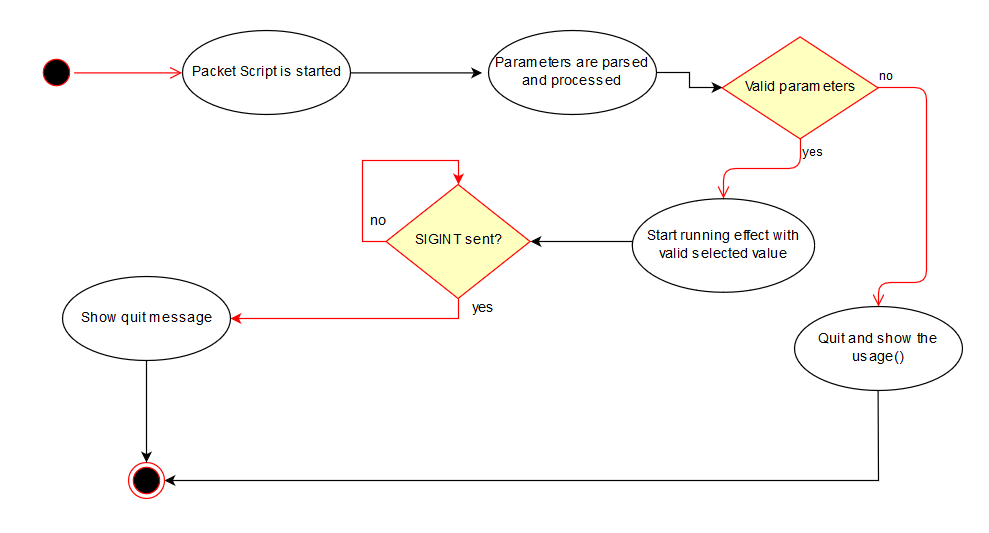
\includegraphics[scale=0.6]{Packet_Activity_Diagram}
	\begin{figure}[h]
		\caption{Activity Diagram for the degradation script}
	\end{figure}
\end{center}

Above is the activity diagram for the packet script that will implement the effect classes above, this script will be utilised directly from the command line or run by the GUI. The decision of having a single script that is controlled by multiple ways allow for one central point of functionality and means code can be shared throughout the project. The activity diagram shows the design choices for the direct control on the script. SIGINT is mentioned in the centre of the diagram, SIGINT is a built in signal in the Linux operating system that represents an interrupt signal, where it is triggered by pressing ``Control + C", this is the most common/clean way of stopping a script. The other alternatives to closing the script ``Control + Z" (SIGTSTP) and ``Control + /" (SIGQUIT) will be remapped to send a SIGINT signal and perform the same role, this will mean the program has one tidy point of closure.




% Section Description:
%
\section{Tool UI Design}
One of the ways mentioned before to control the degradation effects is by a user interface. It needs to have a way to easily add new buttons and text entries that link up to parameters in the script to make the interface scalable and easy to maintain, it also needs a window to display the same output as the terminal window, this can be achieved by `piping' the stdout to a custom section of the user interface. The `stdout' is the data stream that links up to a Linux terminal window, if the stdout points to somewhere else it will display where it is needed. Below is the initial drafted design for the user interface.

\begin{center}
	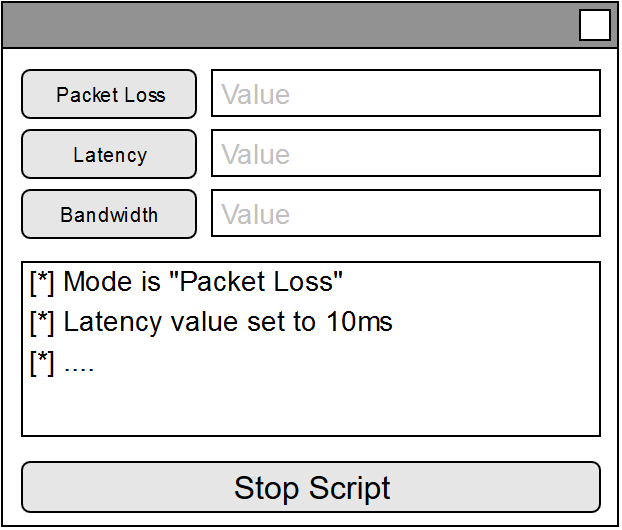
\includegraphics[scale=0.5]{Packet_UI_Design}
	\begin{figure}[h]
		\caption{Initial user interface design for the Degradation GUI}
	\end{figure}
\end{center}



% Section Description:
%
\section{Tool Implementation}

\subsection{NFQUEUE}
The script utilises a section in the Linux kernel referred to as the ``NFQUEUE". This is as the name suggests a queue that is stored in kernel memory that will store up packets until the user provides one of the two verdicts: `Drop' or `Accept'. The packets are pushed into this queue by the use of `iptable' rules, iptabales is a tool designed to filter packets by criteria. Below is a flow diagram for the path a packet might take, each table can have filtering rules embedded into to it:

% Diagram
%Variables
\newcommand{\nodefont}{\rmfamily}
\newcommand{\normalWidth}{3cm}

%----------------------------------------%
%  IPtables Diagram						 %
%----------------------------------------%
\tikzset{%
  >={Latex[width=2mm,length=2mm]},
  % Specifications for style of nodes:
            base/.style = {rectangle, rounded corners, draw=black,
                           minimum width=4cm, minimum height=1cm,
                           text centered, font=\sffamily}, 
            process/.style = {base, minimum width=\normalWidth, fill=orange!15,
                           font=\nodefont},
            network/.style = {base, fill=blue!15},
            local/.style = {base, fill=red!15}}
\vspace{0.25cm}                
\begin{center}
\begin{tikzpicture}[node distance=1.5cm, every node/.style={fill=white, font=\sffamily}, align=center]
    	\node(NetworkCard)[network]{Network Card};
        \node(NetworkCardOut)[network, right of=NetworkCard, xshift=6cm]{Network Card};
        
    	\node(PreRouting)[process, below of=NetworkCard]{Pre-Routing};
    	\node(Forward)[process, right of=PreRouting, xshift=2.5cm, yshift=-1.75cm]{Forward};
    	\node(Input)[process, below of=PreRouting, yshift=-2cm]{Input};
        \node(PostRouting)[process, right of=PreRouting, xshift=6cm]{Post-Routing};
    	\node(Output)[process, right of=Input, xshift=6cm]{Output};
        
        \node(LocalProcessIn)[local, below of=Input]{Local Process};
        \node(LocalProcessOut)[local, below of=Output]{Local Process};
        
        %In Arrows
        \draw[->] (NetworkCard)--(PreRouting);
        \draw[->] (PreRouting)|-(Forward);
        \draw[->] (PreRouting)--(Input);
        \draw[->] (Input)--(LocalProcessIn);
        
        %Out Arrows
        \draw[->] (LocalProcessOut)--(Output);
        \draw[->] (Output)--(PostRouting);
        \draw[->] (Forward)-|(PostRouting);
        \draw[->] (PostRouting)--(NetworkCardOut);        
\end{tikzpicture}
\end{center}   

If there was a case where all packets entering the machine need filtering, an iptable rule would be added to the "Pre-Routing" section of the table to catch all packets entering the machine. 

So for example to move all packets entering from the network card into the NFQUEUE the iptable rule would be added like so:
\begin{center}
	\begin{console_font}
		\large{iptables -A INPUT -j NFQUEUE}
	\end{console_font} 
\end{center}
Where `-a' tells to append a rule onto the `INPUT' table and `-j' is the rule that affects the packet, in this case pushing it into the default queue.

This forms the main component of the functionality of the script, a series of iptable rules that filter packets into the NFQUEUE and allow to script to perform verdicts on each packet separately allows for effects to be easily applied to packets entering and leaving the machine.

Below is code for the creation of the NFQUEUE object along side the iptable rules:
\begin{Code}[]{NFQUEUE}
# iptables
os.system("iptables -A INPUT -j NFQUEUE")
os.system("iptables -A OUTPUT -j NFQUEUE")

# Setup for the NQUEUE
nfqueue = NetfilterQueue()

try:
	nfqueue.bind(0, mode)  # 0 is the default NFQUEUE
except OSError:
	print_force("[!] Queue already created")
	
nfqueue.run()
\end{Code}

In the code above the variable {\code mode} contains a method that performs effects on the packets. An example below shows what {\code mode} would equal if the effect chosen was latency:

\begin{Code}{Latency Packet Mode}
def packet_latency(packet):
    """This function is used to incur latency on packets"""
    if affect_packet(packet):
        assign_thread(latency_obj.effect, [[packet, time.time()]])
    else:
        packet.accept()
\end{Code}

There are a couple of aspect to note in the above code listing:
{\code affect\_packet} is the method that checks the packet against the active filters. {\code assign\_thread} is the method that assigns the object effect method ({\code latency\_obj.effect}) to an idle thread in the pool and 
{\code packet.accept()} and {\code packet.drop()} are the ways the packet is assigned a verdict, this can be done at any point in the code and becomes instantly active.


\subsection{Degradation Effects}
The script contains the functionality to simulate a plethora of effects and each effects functionality will be described below. Please not any of these effects can be chained together in any order.

\subsubsection{Latency}
Latency as described in the background section is the delay in initiating a task and seeing its results. Latency is simulated by using a timing mechanisms where the arrival time of the packet is saved. The packet is then pushed into the NFQUEUE that triggers a single thread that will hold the packet for a set amount of time, the holding time is calculated by taking the amount of time the packet has already been in the script away from the target time. The packet is then marked as `ACCEPTED' and pushed out of the queue.

\begin{Code}{Latency}
def custom_effect(self, packet):
	"""Thread functionality"""

	# # Dynamic time mode
	# Parameters contained within a single object
	if type(packet) is list:
		packetObj = packet[0]
		startTime = packet[1]

		# Works out the time difference between
		# thread conception and now
		elapsed = time.time() - startTime
            
		# Take the elapsed time off the target
		wait_time = self.latency_value - elapsed

		if wait_time < 0:
			pass
		else:
			time.sleep(wait_time)
			self.accept(packetObj)
			
		# # Static time mode
		else:
			time.sleep(self.latency_value)
			self.accept(packet)

\end{Code}

\subsubsection{Packet Loss}
Packet loss is simulated by first assigning a target value, lets say for this example 10\%. For each packet the script randomly generates a number between 1 and 100, if that value is less than the target value the packet is dropped, and if the value is larger the packet is accepted. This therefore creates the effect of packet loss. It does however require a fair amount of packets to balance out statistically and reach the percentage target.

\begin{Code}{Packet Loss}
def custom_effect(self, packet):
        """This function will issue packet loss,
           a percentage is defined and anything
           lower is dropped and anything higher is accepted"""

        if self.packet_loss_percentage != 0:

            # random value from 0 to 100
            random_value = random.uniform(0, 100)

            if self.packet_loss_percentage > random_value:
                self.dropped_packets += 1
                packet.drop()

            # Accept the packet
            else:
                self.accept(packet)
        else:
            self.accept(packet)
\end{Code}

\subsubsection{Bandwidth}
There are two modes created for bandwidth; rate limiting and a simple display. Rate limiting allows the script to limit the rate of bandwidth flowing through the machine and calculates the rate transferred over a period of 5 seconds, if the rate is higher it waits until the rate drops below the target. This gives it the ability to adjust quickly and allows the script to be run for a long period of time without the overall average of the bandwidth affecting future changes. Displaying the bandwidth work exactly the same but without the limit check, this is useful when checking the current download speeds or the max transfer rate.

Limiting bandwidth is below:

\begin{Code}{Bandwidth Limit}
def custom_effect(self, packet):
	"""Used to limit the bandwidth"""

	# Adds packet to the backlog
	self.packet_backlog.append(packet)
	
	# The algorithm will send until the backlog is empty or 
	# the limit is exceeded
	while self.rate < self.bandwidth and len(self.packet_backlog) > 0:
		self.send_packet(self.packet_backlog[0])
            
		# Packet is removed from the list
		del self.packet_backlog[0]
			
		self.calculate_rate_overall_avg()
\end{Code}

\subsubsection{Out-of-order}
This effect changes the order of packets coming into the script, this can be used to check its effect on UDP and TCP and can test how quickly these issue can be rectified. It works by queuing up every packet into a list, then a single thread randomly picks an index of that list, accepts the packet and allows it to leave. This therefore means at its most extreme the order can be last in, first out.

\subsubsection{Connection Simulation}
Connection simulation isn't quite a degradation effect but its intent is to simulate the effect of degradation on a common connection like `WiFi` or a 3G connection to see how these are effected by said degradation. This can be useful in some situations where for example testing a mobile applications performance over 3G with heavy latency, the mobile would connect to the script and the script would effect any traffic entering or leaving the handset.

\subsubsection{Jitter}
Jitter mode clumps and separates packets in their transmission, with some it waits a small period of time other it will clump up delay as a total and then send them all at once. This is to test how the protocol deals with jitter in the connection. Jitter as explained in the background is the intra-packet latency i.e. the difference in time between arrivals of packets.

\subsection{ARP Spoofing}
The script also supports an ARP spoofing mode that allows it to sit between a gateway and a specified target. This means the script can perform all its functions on a single target with a very quick deployment time. As touched on in the background the ARP protocol performs no authentication on any changes to the ARP cache meaning that you can perform a man in the middle attack and route traffic through a machine of your choice.

The script begins by grabbing the MAC addresses connected to the provided gateway and target IP addresses. Two ARP reply packets (denote by the `2' opcode) are sent out: One telling the victim that the current machines MAC address maps to the gateway, and the other telling the gateway that the victims IP maps to the current machines MAC address.

Below is the process visualised:




% Gateway
\newcommand{\GatewayLabel}{
\begin{tabular}{l l}
Gateway\\
\hline
\vspace{0.1cm}
\bf{192.168.1.1} & \bf{C8:49:BD:82:47:4D}\\
ARP Cache\\
\hline
192.168.1.2 & 46:41:73:EC:70:E3
\end{tabular}
}

%Victim
\newcommand{\VictimLabel}{
\begin{tabular}{l l}
Victim\\
\hline
\vspace{0.1cm}
\bf{192.168.1.2} & \bf{46:41:73:EC:70:E3}\\
ARP Cache\\
\hline
192.168.1.1 & C8:49:BD:82:47:4D
\end{tabular}
}

\begin{center}
\begin{tikzpicture}[
    diagram item/.style={},
    align=left
]         

\node (Router)[
    diagram item,
    label=above:\GatewayLabel,
    yshift=-2cm
] {
\includegraphics[scale=\ciscoImageScale]{\cisco/router}};

\node (Victim)[
	diagram item,
	label=above:\VictimLabel,
	right of=Router,
	xshift=7cm
] {
\includegraphics[scale=\ciscoImageScale]{\cisco/workstation}};


\draw[-] (Router)--(Victim);

\end{tikzpicture} 
\end{center}


As you can see both ends are connected and have gone through the process to resolve the IP addresses to MAC addresses, you can see above each device their corresponding IP, MAC and ARP Cache. The ARP cache as mentioned previously is a record linking IP addresses to MAC addresses.

\newcommand{\tgap}{0.1cm}

% Gateway
\newcommand{\GatewayLabelAfter}{
\begin{tabular}{l l}
Gateway\\
\hline
\vspace{\tgap}
\bf{192.168.1.1} & \bf{C8:49:BD:82:47:4D}\\
ARP Cache\\
\hline
192.168.1.2 & \bf{\textcolor{red}{37:A8:22:F6:BB:34}} \\
192.168.1.3 & 37:A8:22:F6:BB:34
\end{tabular}
}

%Victim
\newcommand{\VictimLabelAfter}{
\begin{tabular}{l l}
Victim\\
\hline
\vspace{\tgap}
\bf{192.168.1.2} & \bf{46:41:73:EC:70:E3}\\
ARP Cache\\
\hline
192.168.1.1 & \bf{\textcolor{red}{37:A8:22:F6:BB:34}} \\
192.168.1.3 & 37:A8:22:F6:BB:34
\end{tabular}
}

%Attacker
\newcommand{\AttackerLabel}{
\begin{tabular}{l l}
Attacker\\
\hline
\bf{192.168.1.3} & \bf{37:A8:22:F6:BB:34} 
\end{tabular}
}

\begin{center}
\begin{tikzpicture}[
    diagram item/.style={},
    align=left
]         

\node (Router)[
    diagram item,
    label=above:\GatewayLabelAfter,
    yshift=-2cm
] {
\includegraphics[scale=\ciscoImageScale]{\cisco/router}};

\node (Victim)[
	diagram item,
	label=above:\VictimLabelAfter,
	right of=Router,
	xshift=7cm
] {
\includegraphics[scale=\ciscoImageScale]{\cisco/workstation}};


%Find the middle between the two nodes
\coordinate (CENTER) at ($(Victim)!0.5!(Router)$);		
\node (Attacker)[
	label=below:\AttackerLabel,
	below of=CENTER,
	yshift=-3.5cm
] {
\includegraphics[scale=\ciscoImageScale]{\cisco/laptop}};

\draw[red, very thick] (Router)--(Attacker);
\draw[red, very thick] (Attacker)--(Victim);


\end{tikzpicture} 
\end{center}


Note after the 3rd device connects to the network, both devices gain a record of its IP and MAC address in their ARP cache. 

After both spoofed packets have been send out the ARP cache for each receiving end gets updated, the text in red shows the changes caused by the spoofed ARP packets. Now when either end wants to talk to each other it will resolve the MAC address and send it with the new MAC address in the table, this will therefore get routed through the attacking PC and will allow the script to receive all the traffic between the two parties.

\subsection{Network Attacks}
A couple of network attacks were implemented into the script, these served the purpose of providing very heavy artificial traffic designed to create heavy loads or mess with integral protocols. Not many attacks were added as they don't provide much purpose apart from stress testing and they reside on the edge of the scope of this project. There will also be a brief discussion into possible techniques to mitigate the effects. 

\subsubsection{UDP Flooding}
UDP flooding is a very simple attack, lots of UDP packets are created and send over a network stream very quickly. This attack is designed to `flood' the buffers in the receiving machine and slow down or event prevent internet connection. The script creates 10 or so threads that create and send packet concurrently, this amount of threads easily reaches the max throughput of the test machines NIC card and massively reduces internet connection on the receiving end.

The attack could be detected and prevented by a script that monitors the network transfers rates, this attack will create a huge spike in the transfer rate that can be detected and all traffic would be blocked from the sending party.

\subsubsection{ARP Spamming}
This attack works by once again exploiting the lack of authentication of the ARP protocol. In the entire network mode the script starts by detecting all active hosts on a network, it then starts sending out falsified ARP reply packets with randomly generated MAC addresses inside. This results in all computers on the networking having incorrect ARP cache values and resulting in computers incorrectly resolving IP and MAC address combinations and traffic not being allowed through.

This attack is relatively easy to execute but can simply be prevented by issuing static ARP tables for each machine, this prevents unsolicited ARP replies from changing IP and MAC address combinations and also prevents ARP Spoofing from occurring on that network.


%Experimental design:
%If you project includes any experiments, including but not limited to user testing, then you can discuss their design here. Note that again this does not exist in a vacuum and should be tied to your research.

\section{Test design and system testing}
There are various sections of the project that require a separate testing plan:

\begin{itemize}

	\item Traffic simulation programs\\
	These are the client server programs that will simulate traffic over the synthetic net. These tests will need to 	make 	sure each client and server performs its role correctly.
	
	\item Packet script and effects\\
	This is the script that will run on the custom router. Tests will be checking effects do their basic jobs and the script can be controlled effectively.
	
\end{itemize}

\subsection{Traffic simulation programs}
The test plan for this section will need to check all the intended functionality of each window. There are three aspects of each that will need testing:

\begin{itemize}

	\item UI \\
	Tests will be created that click buttons and check the user interface works effectively through automated testing.

	\item Business Logic \\
	Code behind the UI will have the relevant methods testing with expected and actual results.

	\item Real world usage \\
	The involvement of multiple windows and more complex functionality can be tested by using automated testing 			scripts.
	
\end{itemize}

Appendix A contains the test plan for the program, each separate program has had its user interface and business logic tested and programs that are to be used together have had ``Live" tests created to check their interaction together. The automated tests have been achieved by using the CUIT (Coded User Interface Tests) \footnote{\url{https://msdn.microsoft.com/en-us/library/dd286726.aspx}} that are built into Visual Studio 2017. These allow clicks and movements to be recorded and repeated.

\subsection{Packet Script}
It was decided that a separate test plan was needed for the script that will be run on the router. This was because its design is considerably different to that of the traffic simulation programs. Each individual effect needs a basic test that uses a loopback ping test to simulate incoming traffic where a criteria is looked for, for example to test packet loss, the test pings the script until a packet is lost or a time-out is reached, this can perform a basic test on the functionality of the effect. Each effect will also require validation for the passed parameters, there will be a test created that will test various values inside and outside of the validation range.

\subsection{Testing methodology considerations}
Initially the methodology chosen to start development of the traffic simulation programs was ``Test Driven Development" \citep{beck2003test}, this was a tight methodology that increased development time and gave the added benefit of showing that new changes have not broken older functionality. This methodology was good to start off the project and allowed for a tight structure to be created where no time was wasted debugging previously working code, but as mentioned this methodology slowed development time down, this was chosen to be abandoned after 3-4 weeks to an ad-hoc approach. 
This change was due to time restraints on the project and the less-important role that the traffic simulation programs had on the project compared to the degradation simulation script. The degradation script was developed in the ad-hoc approach, this was due to issue stated previously about the unknown aspects of the script and how it would be operating that it was decided that the time invested to write up test scripts would assume too much and would risk them having the be completely rewritten, tests therefore was added alongside new functionality.





% Section Description
%
\section{Experiential design}
\subsection{Latency Accuracy}
In the initial stages of the project there were experiments that tested the effects of the degradation on the network, the tests were performed on the loopback (Internal network 127.0.0.1) with ICMP ping packets.

This test was designed to show the accuracy of different ways of simulating latency, the first way being a static timer that just causes the thread to sleep for a set amount of time or a dynamic timer that calculates the elapsed time since the creation of the thread and the command telling the thread to sleep, the dynamic timer takes this elapsed time off the target latency value.

Below the results are visualised in a single graph. Please note - the relatively high percentage error in the small ranges of latency this is due to the error proportion being a much larger chunk of the overall target latency and therefore being a higher percentage error:

\begin{tikzpicture}[every axis plot/.append style={thick}]
		\begin{axis}[
			width=\linewidth,
			height=10cm,
			grid=major,
			xmin=1, xmax=100,
			ymin=0, ymax=100,
			xlabel=Latency (ms),
			ylabel=Error (\%)]
			\addplot table [x index=0, y index=1, mark=none, search path=csv_data, col sep=comma]{PingTestDynamicVsStatic.csv};		
			\addlegendentry{Static}	
			
			\addplot table [x index=0, y index=2, mark=none, search path=csv_data, col sep=comma]{PingTestDynamicVsStatic.csv};		
			\addlegendentry{Dynamic}	
		 \end{axis}
 \end{tikzpicture}
 

As you can see from the graph the dynamic form of issuing latency is overall more accurate in simulation, but however, it is still not perfect and there seems to be a small overall error present. This performance is however more than suitable for the scope of this project.

\subsection{Visualising effects}
The most effective way to visualise real world connections were running tests on SpeedTest.net \footnote{\url{http://beta.speedtest.net/}}. This is very useful to quickly visualise a certain effect on the network.

Below are two images showing the effect of a 100ms latency on a networks speed. Both tests were performed on the same empty network and the best result was taken from 5 runs on each.

\begin{center}
	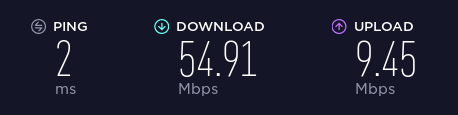
\includegraphics[scale=0.5]{SpeedNoEffect}
	\begin{figure}[h]
		\caption{The initial connection speed}
	\end{figure}
\end{center}

\begin{center}
	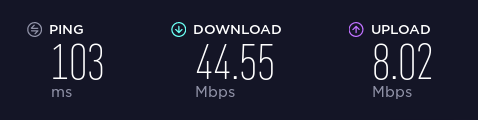
\includegraphics[scale=0.5]{Speed100ms}
	\begin{figure}[h]
		\caption{Network speed with a latency of 100m/s}
	\end{figure}
\end{center}

As you can see from both images, the 100ms has evidently been applied effectively and the speed of the connection has dropped by around 10Mbps. This means in real world terms the time taken to download a 1GB file would take 35 seconds longer to download. This is not a considerable reduction but the latency is having a obvious effect on the network quality.
	%In this chapter you must evaluate your overall project achievement, and provide a clear statement of where the delivered results stand in relation to the original project goals. You should also provide an outline of any further potential work which you can foresee as beneficial to the future development of your project.
\chapter{Evaluation}


%Project Achievements:
%You should consider your original goals and state clearly which have or have not been fully or partially met, and discuss reasons for any significant variance.
\section{Project Achievements}


%UI design:
%If your software includes user interaction then you could also include a discussion (supported by diagrams) of decisions that you have made regarding the user interface.
\section{UI design}

%Further work:
%You should identify any specific areas of the existing product where further work is required, either to address known bugs or omissions, or to improve the system – for example an area you developed at an early stage may in hindsight have been structured in a better way, although it is still perfectly functional.
%You should also provide an outline of any additional areas of potential development you can envisage beyond the initial goals, where the system might be extended in future for greater functionality.
\section{Further work}
	\chapter{Conclusion}

\comments{
The conclusion to your project should contain a summary of your project as you documented it in the preceding text.
It should be clear and concise and include the main contributions of the project.
It often works well to have the conclusion be a matching bookend for the introduction and aims of your project.
}
	%\begin{appendices}

%
\chapter{Test Plan}
\label{ref:testplan}
\small
\begin{longtable}{| p{2cm} | p{0.5cm} | p{4cm} | p{5cm} | p{3cm} |}
	\hline
		%HEADER
		\bf{Section} & \bf{Test No} & \bf{Test Name} & \bf{Description} & \bf{Expected} \\ \hline
		
		%--- UDP CLIENT
		\bf{UDP Client}&&&& \\ \hline
		
		% Business Logic
		Logic &&&& \\ \hline
		&& TestStartUp() & Creates a client object before each test & n/a\\ \hline
		&& TestCleanUp() & No clean-up needed & n/a \\ \hline
		&1& Connect-Disconnect() & The client connects performs no action then disconnects & n/a \\ \hline
		&2& CreateClientObj() & A client object is created & n/a \\ \hline
		&3& SendPacket() & Sends a single UDP packet & n/a\\ \hline
		&4& CheckGridSend() & Checks the method sends out the correct number this depends on grid size & n/a \\ \hline
		
		% UI
		UI &&&& \\ \hline
		&& TestStartUp() & Loads up a fresh window from the command line & n/a \\ \hline
		&& TestCleanUp() & Clicks the X in the top right corner & n/a \\ \hline
		&5& ConnectClick() & Clicks the "Connect" button & n/a \\ \hline
		&6& RestartClick() & Clicks the "Connect" button then the "Restart" button & n/a \\ \hline
		&7& Connect-InvertCheck() & Clicks the "Connect" button and checks all the buttons invert their "Enabled" property correctly & Connect(Disabled), Restart(Enabled) \\\hline
		&8& Restart-InvertCheck() & Clicks the "Connect" button, then the "Reset" button and checks the "Enabled" properties for all buttons are correct & Connect(Enabled), Restart(Disabled) \\\hline
		&9& TextEntry() & Enters text into the text box and then "Connect" is clicked & n/a \\ \hline
				
		%--- UDP SERVER
		\bf{UDP Server} &&&& \\ \hline		
		
		%Business 
		Logic &&&& \\ \hline
		&& TestStartUp() & Creates the client object & n/a \\ \hline
		&& TestCleanUp() & n/a & n/a  \\ \hline
		&10& CreateObject() & Tests that the server object can be created successfully & n/a \\ \hline
		&11& WaitForTimeout() & Starts the server and checks it closes cleanly after time-out & n/a \\ \hline
		
		% UI
		UI &&&& \\ \hline
		&& TestStartUp() & Loads up a fresh window from the CMD line & n/a \\ \hline
		&& TestCleanUp() & Clicks the X in the top right hand corner & n/a  \\ \hline
		&12& StartClick() & Click the "Start" button & n/a \\ \hline
		&13& RandomiseClick() & Click the "Randomise" button & n/a \\ \hline
		&14& Start-ResetClick() & Clicks the "Start" button then resets and checks it returns to it's default state & n/a \\ \hline
		&15& Randomise-ResetClick() & Clicks the "Randomise" button, the resets and checks it returns to it's default state & n/a \\ \hline
		&16& Start-CheckInvert() & "Start" button clicked and then the test checks for "Enabled" property is inverted & n/a \\ \hline
		&17& RestartCheckInvert() & "Start" then "Restart" button clicked and the test then checks for the correct inverting of the buttons "Enabled" property Start = Enabled, Restart = Disabled & n/a \\ \hline
		&18& Stat-PacketLossReset() & Checks when the restart button is clicked the statistics is returned to default & "-" \\ \hline
		&19& Stat-TotalPacketLossReset() & Checks when the restart button is clicked the statistics is returned to default & "-" \\ \hline
		&20& Stat-TotalPacketSentReset() & Checks when the restart button is clicked the statistics is returned to default & "-" \\ \hline
		&21& Stat-CheckDeafult() & "Start" is clicked and the test then waits for a time-out, it then checks the default values of the statistics & PacketLoss(100) \\ \hline
		
		%--- UDP COMBINED		
		Live Tests &&&& \\ \hline
		&& TestStartUp() & Both windows were opened on the command line & n/a \\ \hline
		&& TestCleanUp() & Both windows are closed by automated actions & n/a \\ \hline
		&22& SendAndRecieve-Valid() & The client sends packages to the server and the server accepts packets & n/a \\ \hline
		&23& SendAndRecive-Valid-Twice() & The performs the same action at the above test but does the whole loop an extra time to check if the reset works correctly & n/a \\ \hline
		&24& SendAndRecieve-Invalid() & This test doesn't connect the client to the server but a random IP on the network, this is to check the server will act accordingly & n/a \\ \hline

		\bf{FTP Server} &&&& \\ \hline
		
		%--- FTP Logic
		Logic &&&& \\ \hline
		&& TestStartUp() & Creates the server object & n/a \\ \hline
		&& TestCleanUp() & n/a & n/a \\ \hline
		&25& CreateObject() & Creates a version of the server object & n/a \\ \hline
		&26& ServerSetup() & Performs the server set-up & n/a \\ \hline
		&27& ServerStart() & Sets up the server and starts it & n/a \\ \hline
		&28& ServerStartStop() & Does a fully cycle for the server & n/a \\ \hline
		
		%--- FTP Combined
		&& TestStartUp() & Loads up FTP Server and FileZilla & n/a \\ \hline
		&& TestCleanUp() & Closes each window with automated actions & n/a \\ \hline
		&& ValidConnection() & Automated UI test that simulates a valid connection and checks elements on the UI for signs of a valid connection & n/a \\ \hline
		&& InvalidConnection() & Test that attempts to connect to a non working server & n/a \\ \hline
		&& DownloadFile() & A test that simulates a download of a file and checks it completes fully & n/a \\ \hline
		&& InteruptDownload() & Test that starts a download and interrupts it before completion & n/a \\ \hline
	\hline
\end{longtable}

Packet Script Test Plan for the default effects.

\begin{longtable}{| p{2cm} | p{0.5cm} | p{4cm} | p{5cm} | p{3cm} |}
	\hline	
	\bf{Section} & \bf{Test No} & \bf{Test Name} & \bf{Description} & \bf{Expected} \\ \hline
	\bf{Effects} &&&& \\ \hline
	PacketLoss &&&& \\ \hline
	&1& StartPacketLoss() & Starts the script with the expected parameter (e.g. -pl 10) &  Script should start PacketLoss mode \\ \hline
	&2& PacketLossEffect() & Pings the script and checks the effect on the ping packets, the test pings until one packet is lost. Checking for exact percentages isn't reliable enough & Some packet loss \\ \hline	
	Latency &&&& \\ \hline
	&3& StartLatency() & Starts the script with valid parameters for latency (e.g. -l 10) & Script should start in Latency mode \\ \hline
	&4& LatencyEffect() & Pings the script and checks the latency value within a margin of error & Latency effect on ping packets \\ \hline	
	Bandwidth &&&& \\\hline
	&5& StartBandwidth() &  Starts the script with the expected parameters (e.g. -rl 100) & Script should start in Bandwidth limit mode \\ \hline
	&6& BandwidthEffect() & Starts bandwidth mode and starts pinging the localhost, after a certain amount of packets the rate is calculated and checked against the rate limit value & n/a \\\hline
	Script &&&& \\ \hline
	&7& LatencyValidation() & Check that the validation works for the latency mode & Range = 1-1000ms \\\hline
	&8& PacketLossValidation() & Check that the validation works for the packet loss mode & Range = 1-100\%\\\hline
	&9& BandwidthValidation() & Checks that validation works for bandwidth mode & Range =  1-10000B/s\\\hline
	
\end{longtable}

%
\chapter{GitHub Issues}
\begin{center}
	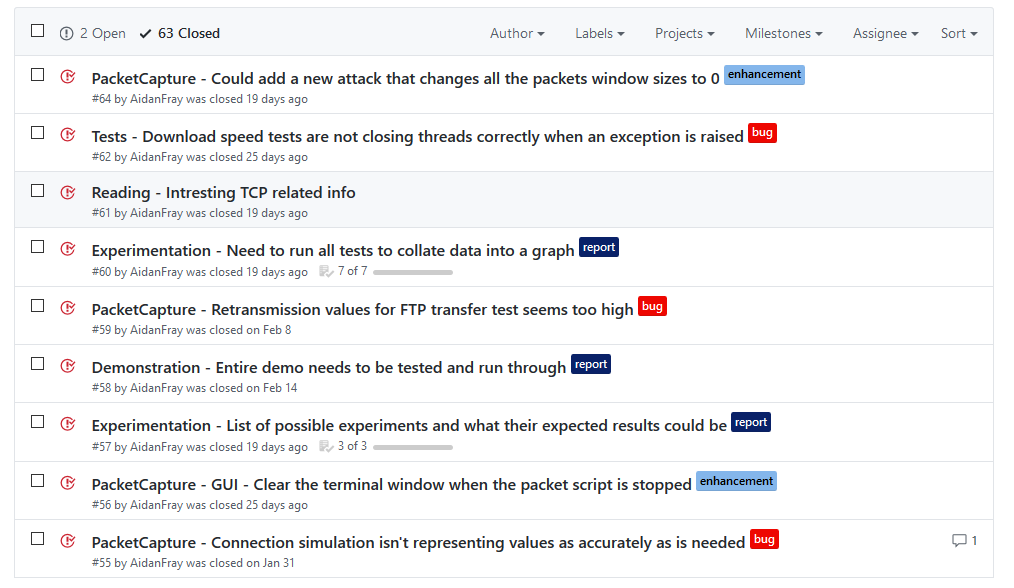
\includegraphics[scale=0.6]{github_issues}
	\begin{figure}[h]
		\caption{Snapshot of actual issues created in the project}
		\label{ref:GitHubIssues}
	\end{figure}			
\end{center}

\begin{center}
	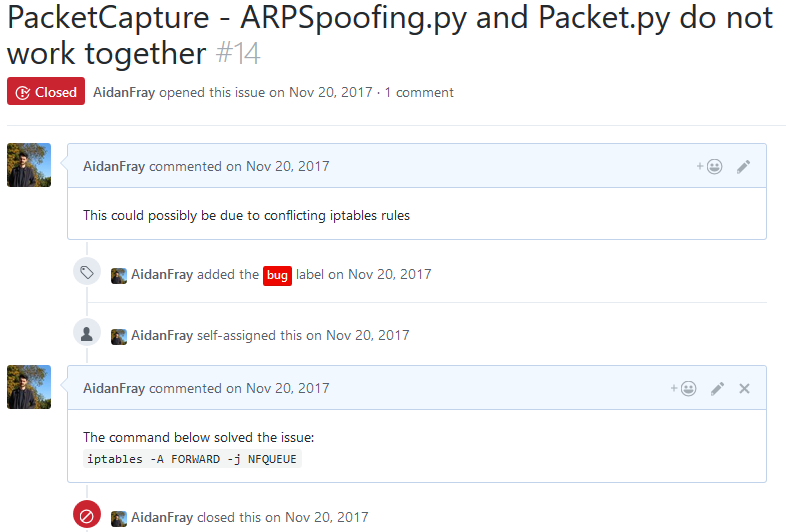
\includegraphics[scale=0.6]{github_issue_des}
	\begin{figure}[h]
		\caption{Example of an issue with discussion}
		\label{ref:GitHubIssueExample}
	\end{figure}	
\end{center}

%
\chapter{Testing Correctness}
\begin{center}
	\label{ref:testingCorrect}
	\begin{tabular}{| p{3cm} | p{5cm} | p{1cm} |}
	
	\lineend
	%--- UDP CLIENT
	\header{UDP Client}\lineend
	
	\bf{Logic} && \\ \lineend
	UC-L3	& Connect-Disconnect() 			& \Pass \\ \lineend
	UC-L4	& CreateClientObj() 			& \Pass \\ \lineend
	UC-L5	& SendPacket() 					& \Pass \\ \lineend
	UC-L6	& CheckGridSend() 				& \Pass \\ \lineend
	
	\bf{UI} && \\ \lineend	
	UC-U3 	& ConnectClick() 				& \Pass \\ \lineend
	UC-U4	& RestartClick() 				& \Pass \\ \lineend
	UC-U5	& Connect-InvertCheck() 		& \Pass \\ \lineend
	UC-U6	& Restart-InvertCheck() 		& \Pass \\ \lineend
	UC-U7	& TextEntry() 					& \Pass \\ \lineend
	
	%--- UDP Server
	\header{UDP Server}\lineend
	
	\bf{Logic} && \\ \hline
	US-L3	& CreateObject() 				& \Pass \\ \lineend
	US-L4	& WaitForTimeout() 				& \Pass \\ \lineend	
	
	\bf{UI} && \\ \lineend
	US-U3	& StartClick()					& \Pass \\ \lineend
	US-U4	& RandomiseClick() 				& \Pass \\ \lineend
	US-U5	& Start-ResetClick() 			& \Pass \\ \lineend
	US-U6	& Randomise-ResetClick()		& \Pass \\ \lineend
	US-U7	& Start-CheckInvert() 			& \Pass \\ \lineend
	US-U8	& RestartCheckInvert() 			& \Pass \\ \lineend
	US-U9	& Stat-PacketLossReset()		& \Pass \\ \lineend
	US-U10	& Stat-TotalPacketLossReset() 	& \Pass \\ \lineend
	US-U11	& Stat-TotalPacketSentReset() 	& \Pass \\ \lineend
	US-U12	& Stat-CheckDeafult()		  	& \Pass \\ \lineend
		
	\header{UDP Combined}\lineend
	\bf{Live} && \\ \lineend
	U-3		& SendAndRecieve-Valid() 		& \Pass \\ \lineend
	U-4		& SendAndRecive-Valid-Twice() 	& \Pass \\ \lineend
	U-5		& SendAndRecieve-Invalid() 		& \Pass \\ \lineend	
	
\end{tabular}

	\begin{figure}[h]
		\caption{Testing correctness for the UDP Server and Client}
		\label{ref:testingUDP}
	\end{figure}
	
	\begin{tabular}{| p{3cm} | p{5cm} | p{1cm} |}

\lineend
\header{PacketLoss}
P-1		& StartPacketLoss() 		& \Pass \\ \lineend
P-2		& PacketLossEffect()		& \Pass \\ \lineend

\header{Latency} 
L-1		& StartLatency() 			& \Pass	\\ \lineend
L-2		& LatencyEffect() 			& \Pass \\ \lineend

\header{Bandwidth} 
B-1		& StartBandwidth()			& \Pass \\ \lineend	
B-2		& BandwidthEffect() 		& \Pass \\ \lineend

\header{Out-Of-Order}
O-1		& StartOrder()				& \Pass \\ \lineend
O-2		& OutOfOrderEffect()		& \Pass \\ \lineend

\header{Jitter}
J-1		& StartJitter()			 	& \Pass \\ \lineend
J-2		& JitterEffect() 			& \Pass \\ \lineend

\header{Validation} 
V-1		& LatencyValidation() 		& \Pass \\ \lineend
V-2		& PacketLossValidation() 	& \Pass \\ \lineend
V-3		& BandwidthValidation()	 	& \Pass \\ \lineend
V-4		& OutOfOrderValidation()	& N/A 	\\ \lineend
V-5		& JitterValidation()		& \Pass \\ \lineend
\end{tabular}
	
	\begin{figure}[h]
		\caption{Testing correctness for the main script functions}	
		\label{ref:testingScript}
	\end{figure}
\end{center}
\end{appendices}

	
	%\bibliographystyle{hull}
	%\bibliography{report}
	
\end{document}
